
\section{Motores}  \label{secao_motores}

\subsection{Motores DC}

Durante os estudos e testes foi usado por um tempo motores DC com encoder.
Os motores são do modelo CHR\_GM25\_370 6v e 210rpm, fabricado por Shenzhen Chihai Motor,
de acorco com \cite{motor_dc_6v_encoder}, é um motor de imã permanente.
Essa escolha inicial foi motivada pela simplicidade de uso para o motor operar um motor DC.
Porém controlar o motor DC de imã permanente trouxe uma série de desafios.
O motor possui uma caixa de redução de 1:34. Tal motor possui um encoder magnético acoplado, com 11
PPR (\textit{``Pulses Per Revolution''}), resultando em um encoder com resolução de 374 PPR.

Esse encoder prodruz duas ondas quadradas como saídas, A e B \cite{encoder_ppr}.
As duas possuem 90° de fase entre si,
e, caso a onda A esteja adiantada em relação a B (\autoref{encoder_ppr_ab}),
o sentido de rotação é positivo (anti-horário).

% LUCAS.
% Incluir um pouco sobre a diferença sobre os tipos de motores DC, mas não muito, pouca coisa
% um paragrafo pequeno é suficiente
% https://www.aarohies.com/what-is-the-difference-between-pmdc-bldc-and-pmsm-motor/
% https://www.monolithicpower.com/en/learning/resources/brushless-vs-brushed-dc-motors
% https://techweb.rohm.com/product/motor/brushed-motor/209/


\begin{figure}[ht]
	\centering
	\caption{Motor DC 6V}
	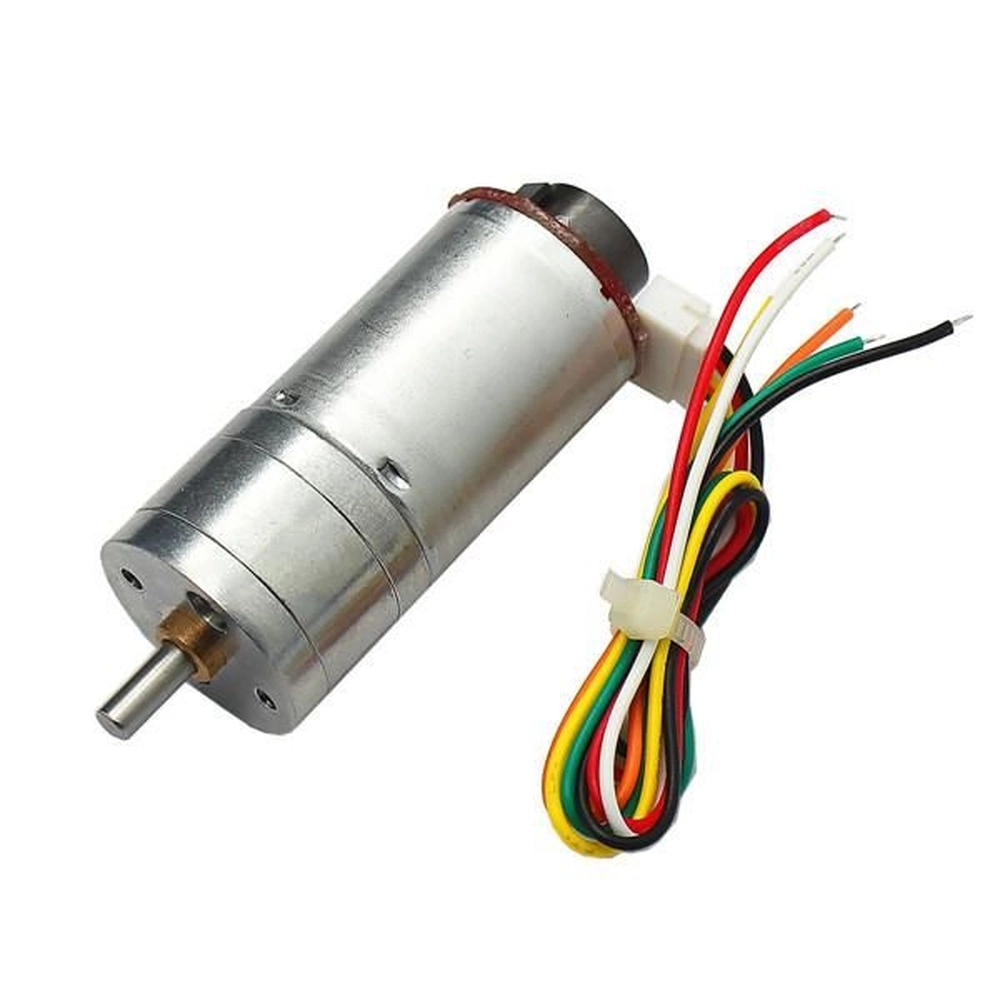
\includegraphics[width=0.7\textwidth]{figures/CHR_GM25_370}
	\fonte{\cite{motor_dc_6v_encoder}}
\end{figure}

\begin{figure}[ht]
	\centering
	\caption{Encoder holzer}
	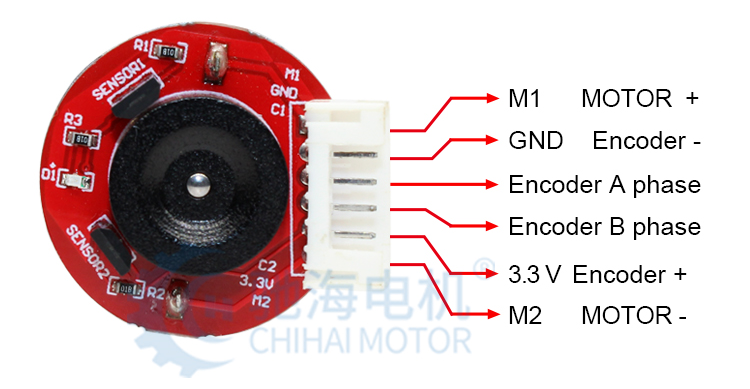
\includegraphics[width=0.5\textwidth]{figures/encoder_holzer}
	\fonte{\cite{motor_dc_6v_encoder}}
\end{figure}

\begin{figure}[ht]
	\centering
	\caption{Ondas quadradas resultantes dos pulsos de saída do encoder}
	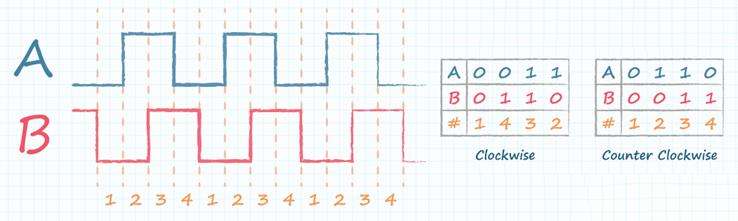
\includegraphics[width=1\textwidth]{figures/encoder_pulso_ab}
	\fonte{Adaptado de \cite{encoder_ppr}}
	\label{encoder_ppr_ab}
\end{figure}


\subsubsection{Controle de velocidade}

\subsubsubsection{Medição de velicidade do motor}

Como encoder possuí dois sinais de onda quadadra defasadas em 90º, fase A e fase B, cujos vales e picos são valores lógicos HIGH e LOW, 
e direção de rotação do motor pode ser definida pela diferença entre as fases, se fase A esta adiantada ou atrasada em relação a fase B
É possível calcular a velocidade com base nas subidas da onda quadrada de uma fase, e o valor logico da outra fase no momento da subida.
Por exemplo,  observando a fase B, toda vez em que há uma subida, se o valor da fase A for alto, então incrementar +1 em um contador, se a fase A tiver valor baixo, então incrementar -1 no contador.
Quando o valor da fase A for alto, então o motor esta rodando em um sentido,  quando o valor  for baixo, então o motor esta rodando no sentido contrário.
Medindo o valor do contador por um $\Delta_{T}$, se resulta na quantidade de pulsos por segundo.
Para converter de pulsos por segundo para RPM, basta dividir pela resolução do motor+encoder,  que é de 1:34 do motor, e 11 pulsos por rotação do encoder, o que resulta em 374,
e multiplicar por 60 para ter o resultado em rotações por minuto.

\begin{figure}[ht]
    \centering
    \caption{Interpretação gráfica do método de leitura do encoder}
	\begin{tikzpicture}[node distance=1.5cm, scale=1, every node/.style={scale=0.6}]
		\node (start) [startstop] {início loop};
		\node (pro1) [process, below of=start] {ENQUANTO DELTA T};
		\node (in1) [io, right of=pro1, xshift= 4cm] {QUANDO FASE B = SUBIDA};
		\node (dec1) [decision, below of=in1, yshift=-2cm] {SE FASE A = 1};
		\node (pro1a) [process, below of=dec1, yshift= -2cm] {INCREMENTAR CONTADOR em +1};
		\node (pro1b) [process, right of=dec1, xshift= 3cm] {INCREMENTAR CONTADOR em -1};
		\node (count) [process, below of=pro1, yshift= -7cm] {CONTADOR DIVIDO POR DELTA T};
		\draw [arrow] (start) -- (pro1);
		\draw [arrow] (pro1) -- node[anchor=north] {sim} (in1);
		\draw [arrow] (in1) -- (dec1);
		\draw [arrow] (dec1) -- node[anchor=east] {sim} (pro1a);
		\draw [arrow] (dec1) -- node[anchor=north] {não} (pro1b);
		\draw [arrow] (pro1) -- node[anchor=east] {não} (count);
	\end{tikzpicture}
    \fonte{Própria}
    \label{fluxograma_cencoder}
\end{figure}


Na implementação dessa lógica no STM32, o desafio foi a definição do $\Delta_{T}$,
Se o $\Delta_{T}$ for muito pequeno, o resultados de pulsos por segundo pode tender ao infinito, gerando valores muito altos.
No lado esquerdo da \autoref{medidas_altas} em laranja, esta o resultado do rpm considerando o $\Delta_{T}$ como o tempo entre os ciclos do micrcontrolador.
A outra opção, foi definir um $\Delta_{T}$ fixo, definindo uma frequencia de medição pré definida,
e o resultado pode ser visto em azul no lado esquerdo na \autoref{medidas_altas}
Essa outra opção de $\Delta_{T}$ resultou em um sinal que tem uma componente em alta frequência com uma amplitude até consideral.
Analisando os dois sinais no dominio da frequêcia no lado direto da \autoref{medidas_altas},
o espectro em frequência do sinal em laranja possui amplitudes muitos semelhante em todo espectro,
mas o espectro do sinal em azul, fica bem claro que em altas frequencias é composto mais por ruidos
e as frequencia médias tem amplitude menor em relação as frequências baixas,
o que torna mais fácil aplicar um filtro passa-baixa para reduzir as frenquências médias e altas.

\begin{figure}[ht]
    \centering
    \caption{Medidas do encoder}
    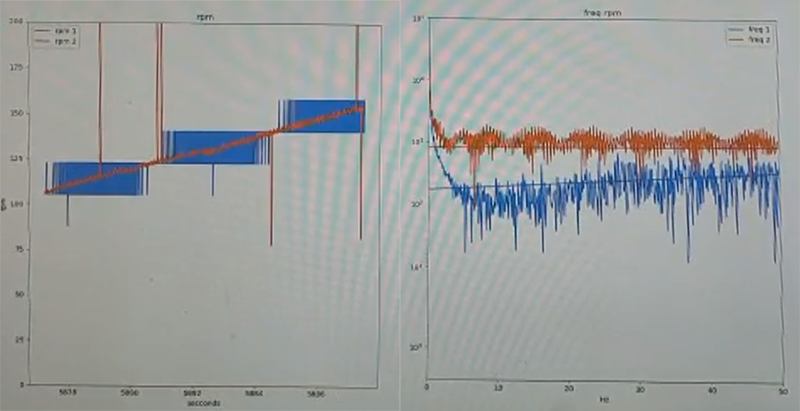
\includegraphics[width=1\textwidth]{figures/medidas_altas}
    \fonte{Própria}
    \label{medidas_altas}
\end{figure}


A \autoref{passa_baixa_teste}, mostra um dos teste de filtro passa baixa,
em o sinal em laranja ainda persiste esses valores tentendo ao infinito, 
devido a ampliture eles se tornam um pouco dificil de serem retirados.
Mas o sinal em azul acaba tendo um resultado melhor depois do filtro, muito semelhando ao sinal em laranja.
Com base nesse resultado, foi decidido seguir com o método em que o $\Delta_{T}$ é definido por uma frequência pré definida.

\begin{figure}[ht]
    \centering
    \caption{Teste de filtro passas-baixa}
    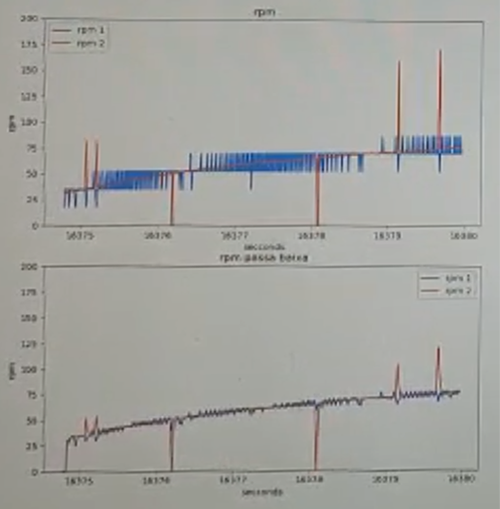
\includegraphics[width=0.6\textwidth]{figures/passa_baixa_teste}
    \fonte{Própria}
    \label{passa_baixa_teste}
\end{figure}


Com o método definido, foi definido um $\Delta_{T}$ em 100hz eu um filtro passa baixa em 2hz.
A equação \eqref{equacao_diferenca} a seguir é a equação de diferença do filtro, considerando uma amostragem de 100hz e frequência de corte em 2hz.

\begin{equation}
    \begin{split}
        y[k] = 0.0591174 \cdot u \left[ k \right] +  0.0591174 \cdot u[k - 1] + 0.88176521 \cdot y[k - 1]
    \end{split}
    \label{equacao_diferenca}
\end{equation}

\subsubsection{Curva PWM x RPM - problema da não linearidade}

Depois de definido como calcular a velocidade o próximo desafio foi lidar com a não linearidade entre o PWM e o resultado medido em RPM.
Como pode ser visto na figura \autoref{grafico_pwm_x_rpm}, na comparação entre o valor do PWM e o RPM no tempo.

\begin{figure}[ht]
	\centering
	\caption{Curva PWM e RPM no tempo}
	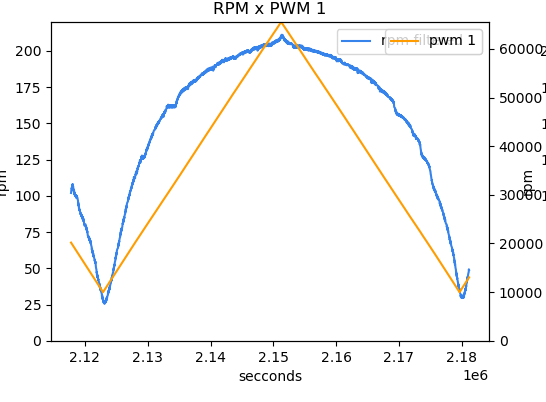
\includegraphics[width=0.6\textwidth]{figures/pwm_x_rpm}
    \fonte{Própria}
	\label{grafico_pwm_x_rpm}
\end{figure}

Considerando essa não linearidade, foram realizadas 15k medições em PWM vs RPM para definir uma equação que pudesse relacionar o PWM com o RPM.
Como pode ser observado no gráfico ``Curva PWM x RPM dados brutos'' na \autoref{medicao_pwm_x_rpm},
os resultados possuem uma tendência, mas possuem alguns pontos fora da curta.
devido ao esses ruídos nas medições ss dados foram tratatos para obter valores médios dos resultados usando python.

\begin{figure}[ht]
	\centering
	\caption{Curva PWM x RPM dados brutos}
	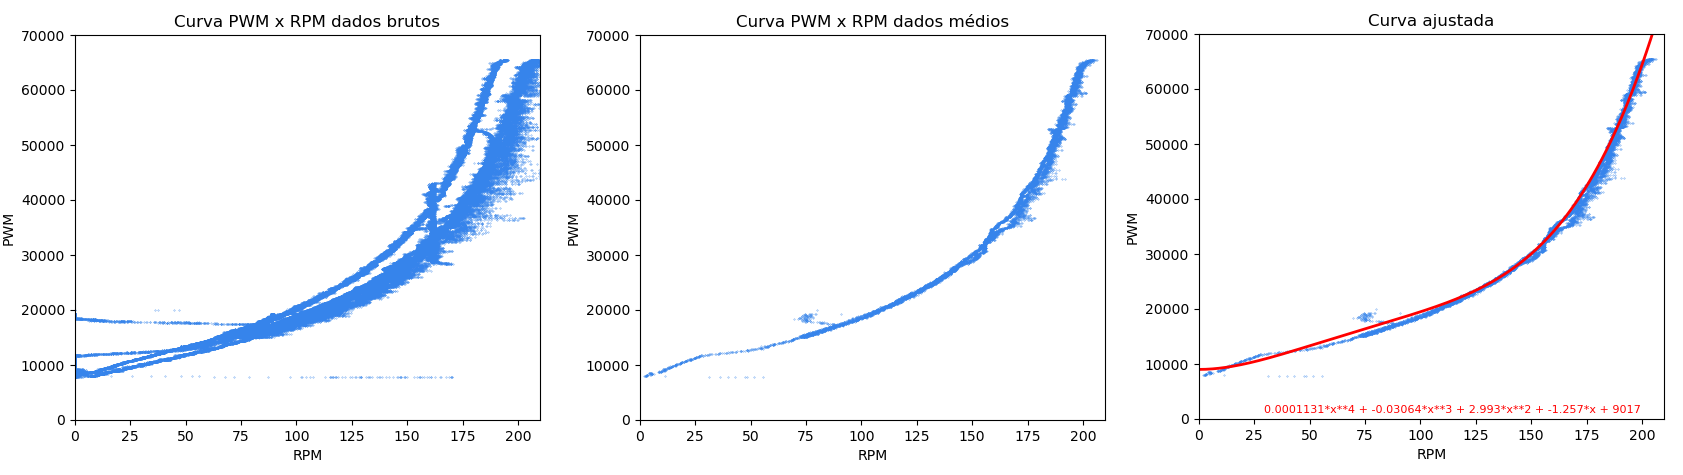
\includegraphics[width=1\textwidth]{figures/curva_pwm_x_rpm_dados}
    \fonte{Própria}
	\label{medicao_pwm_x_rpm}
\end{figure}

O resultado da limpeza dos dados pode ser vizualizado no gráfico ``Curva PWM x RPM dados médios'' na \autoref{medicao_pwm_x_rpm}.
Após a limpeza dos dados, os dados foram importados para o matlab, 0anexo \ref{anx_matlab},
para obter um polinômio que possa definir a curva, o polinômio resultante é a equação \eqref{polimonio_rpm},
e o gráfico ``Curva ajustada'' na \autoref{medicao_pwm_x_rpm} representa a curva ajustada.
A equação do polinômio foi inserida no código do micrcontrolador, foi testado definir um RPM de 150,
e a tabela \ref{medicao_motores} trás uma amostra dos resultados dos RPMs de cada motor.
Com essa equação é mais fácil definir um comportamento linear, facilitando a aplicação de um controle PDI.

\begin{equation}
    \begin{split}
        0.0001131x^{4} + -0.03064x^{3} + 2.993x^{2} + -1.257x + 9017
    \end{split}
    \label{polimonio_rpm}
\end{equation}

\begin{table}[ht]
    \centering
	\caption{Medição rpms motores}
	 \begin{tabular}{|c|c|c|c|c|}
		\hline
		\textbf{$Tempo_{seg}$} & \textbf{$RPM_{definido}$} & \textbf{$RPM_{medido_{1}}$} & \textbf{$RPM_{medido_{2}}$} & \textbf{$RPM_{medido_{3}}$} \\ \hline
		52.954 & 150.00  & 141.03 & 162.69 & 149.82 \\ \hline
		52.954 & 150.00  & 141.43 & 162.43 & 149.18 \\ \hline
		53.000 & 150.00  & 140.83 & 162.19 & 148.61 \\ \hline
		53.000 & 150.00  & 140.30 & 161.98 & 149.06 \\ \hline
		53.000 & 150.00  & 140.79 & 161.80 & 149.46 \\ \hline
		53.000 & 150.00  & 141.21 & 161.64 & 148.86 \\ \hline
		53.046 & 150.00  & 141.59 & 161.49 & 149.28 \\ \hline
		53.046 & 150.00  & 141.92 & 161.37 & 149.65 \\ \hline
		53.046 & 150.00  & 141.26 & 161.25 & 149.02 \\ \hline
		53.046 & 150.00  & 140.68 & 162.11 & 148.48 \\ \hline
		53.046 & 150.00  & 141.12 & 162.86 & 148.94 \\ \hline
		53.092 & 150.00  & 141.51 & 162.57 & 149.35 \\ \hline
		53.092 & 150.00  & 141.85 & 162.32 & 148.76 \\ \hline
		53.092 & 150.00  & 141.20 & 162.09 & 149.19 \\ \hline
		53.092 & 150.00  & 140.63 & 161.90 & 149.57 \\ \hline
	\end{tabular}
	\fonte{Própria}
	\label{medicao_motores}
\end{table}


\subsubsubsection{Implementação da medição de rpm e filtro passa baixa no microcontrolador}

Para medir a velocidade de um motor DC com base no encoder, foi necessário realizar a leitura das subidas dos calores de LOW para HIGH de uma das fases do enconder, e comparar com outra Fase
Para isso usamos o sistema de interrupção do microcontrolador.
O algortimo precisa registrar em um contador a quantidade de pulsos de uma fase, 
depois calcular a taxa de pulsos por segundo, usando o diferencial da velocidade no dominio discreto, $\Delta$p/$\Delta$t.
Porém calcular velocidade a cada ciclo do micrcontrolador acaba registrando valores de tempo muito pequenos, fazendo a velocidade tender ao infinito
A solução foi estabelecer uma amostragem do registro da velocidade, porem a amostragem adiciona um ruido com frequências maiories que do sinal original e de amplitude definida.
Para retirar essas frequência do sinal, o filtro passa baixa foi implementado pelo código que esta no \ref{anx_passa_baixa}


\subsubsection{Decisão final sobre os teste com motor DC}

Durante os teste, os motores não possuem torque o suficiente para dar partida em baixas velocidades,
Seria necessário programar no microcontrolador um sistema de partida para os motores receberem corrente o suficiente
para dar partida em baixas velocidades
Somando a complexidade do algoritimo para controlar um motor DC de imã permanente, foi necessário repensar o tipo de motor.
Para esse tipo de controle preciso de velocidade, foi consdirado mudar para motores de passo, um NEMA 17 bipolar.
Popular em impressoras 3D, seu custo de venda é mais barato devido a maior disponibilidade.
Outro motivo que levou a escolha, foi o fato de serem motores de reposição de uma impressora 3D usada no projeto.

\subsection{Motores de passo}

Os motores de passo operando em passos por segundo, o controle de velocidade é mais fácil,
e as possíveis variações de rpm ocorrem a nível de ciclos do microcontrolador.

Porém motores de passo exigem um cuidado maior, além de exigem uma alimentação maior, de 12v a 24v, os uso dos drivers para motor de passo exigem um maior cuidado na montagem.

\begin{figure}[htb]
	\centering
	\caption{Motor de passo Nema 17}
	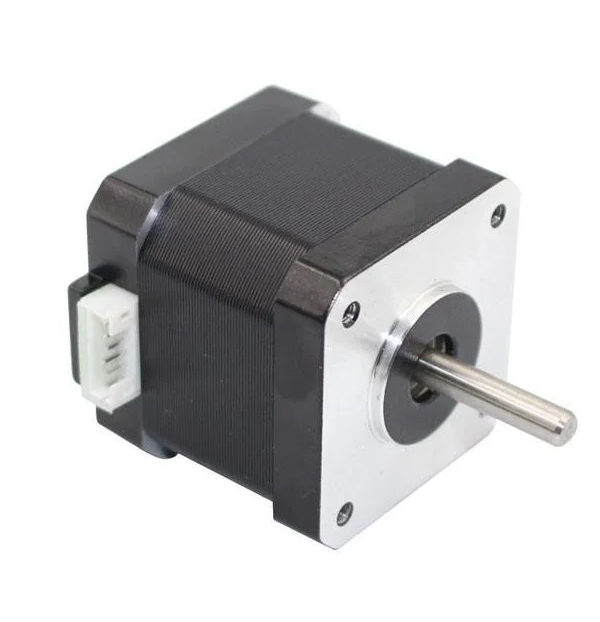
\includegraphics[width=0.7\textwidth]{figures/JK42HS40_1704_13A}
	\fonte{\cite{motor_dc_6v_encoder}}
	\label{Especificacoes_motordc_6v}
\end{figure}

\begin{table}[ht]
	\centering
	\caption{Especificações do motor DC 6V}
	 \begin{tabular}{|c|c|c|c|}
		\hline
		\textbf{Especificação} & \textbf{Valor} \\ \hline
		Corrente por fase & 1.7A  \\ \hline
		Torque nomimal  & 4.2 KGF (~46 N) \\ \hline
		Angulo de passo & 1.8° \\ \hline
		Polaridade & bipolar \\ \hline
	\end{tabular}
	\fonte{\cite{motor_dc_6v_encoder}}
	\label{Especificacoes_motordc_6v}
\end{table}


Outro desafio do motor de passo é idenfiticar as fases, pois cada fabricante pode ter uma ordem diferente dos pinos de saida do motor.
Para idenfiticar quais pinos compõem cada fase, bastou verificar com o multimetro quais fases estavam em curto.
Restando identicar somente o pontos A e B de cada fase de acordo com o diagrama a seguir.

\begin{figure}[htb]
	\centering
	\caption{Motor de passo - Fases Bipolar \cite{motor_dc_6v_encoder}}
	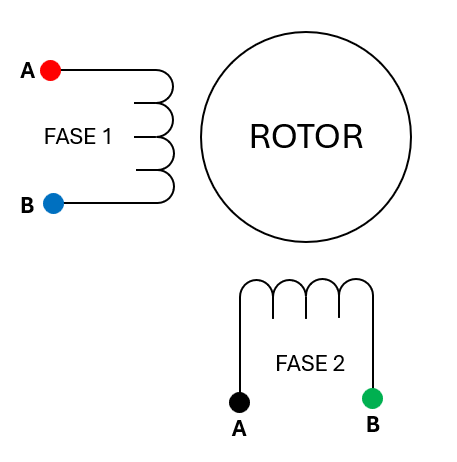
\includegraphics[width=0.7\textwidth]{figures/motor_wiring}
	\fonte{\cite{motor_dc_6v_encoder}}
	\label{Especificacoes_motordc_6v}
\end{figure}

Para identificar quais eram os pontos A e B de cada fase, foi necessário um processo de tentantiva e erro,
para relacionar o diagrama de fases com os pinos do motor, e o resultado esta ilustrado na figura \ref{nema_pinout}

\begin{figure}[htb]
	\centering
	\caption{Motor de passo - Idetificação dos pinos}
	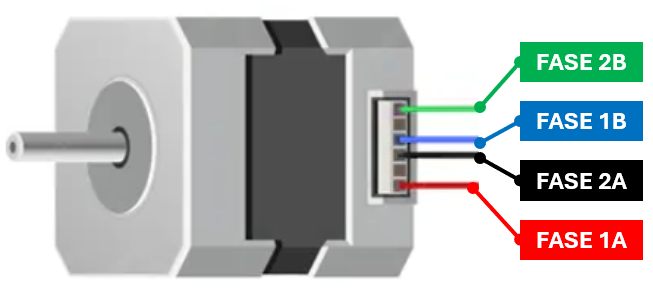
\includegraphics[width=0.7\textwidth]{figures/motor_pinout}
	\fonte{\cite{motor_dc_6v_encoder}}
	\label{nema_pinout}
\end{figure}
